\documentclass[italian]{beamer}
%\documentclass[italian,handout]{beamer}

\usepackage[utf8]{inputenc}

\title[Bitcoin]{Analisi di Bitcoin}
\subtitle{Anonimato, Sicurezza e Sviluppi Futuri}
\author[Paoluzzi Matteo]{Paoluzzi Matteo}
\institute[UniUD]{Università degli Studi di Udine\and{}Relatore:\\{}Dott. Ivan Scagnetto}
\date[2014/04/03]{IV Sessione di Laurea AA 2012/2013, Aprile 2014}
\subject{Bitcoin}

\usepackage{default}
\usepackage{pres_commands}
%\usepackage{pres_uniudtesi}
\usetheme{Madrid}

\graphicspath{{./img/}}

\hypersetup{
  pdfstartview={Fit},
  pdftitle={Presentazione della Tesi ``Analisi di Bitcoin: Anonimato, Sicurezza e Sviluppi Futuri``},
  pdfauthor={Paoluzzi Matteo},
  pdfsubject={Modello di presentazione di Tesi al computer},
  pdfkeywords={LaTeX pdf presentazione tesi laurea}}

\begin{document}

\frame{\titlepage}

\begin{frame}{Di cosa si tratta} % 1
Una valuta elettronica basata su crittografia a chiave pubblica progettata per:
\begin{itemize}
 \item Proteggere l'identità degli utenti sfruttando \textbf{indirizzi} anonimi.
 \item Essere indipendente da qualsiasi istituto di credito.
 \item Essere immune dal rischio di inflazione.
 \item Funzionare su base P2P in modo pubblico, sicuro e verificabile.
\end{itemize}
\end{frame}

\begin{frame}{Indirizzi} % 2
L'anonimato dell'utente viene implementato tramite stringhe di testo note come indirizzi.
\begin{itemize}
 \item Un indirizzo viene generato a partire da una coppia di chiavi pubbliche e private.
 \item Tutte le \textbf{transazioni} di BTC avvengono da e verso indirizzi, senza divulgare informazioni sull'identità delle parti coinvolte.
 \item Le chiavi di cifratura consentono di spendere il denaro ricevuto e impedire che il denaro inviato finisca ad un destinatario diverso da quello desiderato.
 \item Ogni utente è incoraggiato ad avere molteplici indirizzi, mantenendo sicure le porzioni private delle chiavi appositamente generate.
\end{itemize}
\end{frame}

\begin{frame}{Transazioni} % 3
Contengono tutte le informazioni necessarie per effettuare un ''trasferimento`` di denaro.
\begin{itemize}
 \item Sono identificate da un hash calcolato su un suo sottoinsieme di dati che ne cristallizzano le proprietà più rilevanti.
 \item Contengono molteplici sezioni di input e output costituite da script eseguibili che autorizzano la spesa e determinano l'invio del denaro:
 \begin{itemize}
  \item L'input contiene un riferimento ad output di precedenti transazioni da cui prelevare denaro, e per ogni riferimento la chiave pubblica del creatore della transazione attuale e la relativa firma ECDSA che ne autorizzano il prelievo.
  \item Ogni output contiene un ammontare in denaro e uno script con l'indirizzo del destinatario che autorizzerà future spese della transazione.
  \item Se l'input è maggiore dell'output, il resto viene inviato ad un indirizzo scelto dal creatore della transazione.
 \end{itemize}
\end{itemize}
\end{frame}

\begin{frame}{Blocchi} % 4
Le transazioni vengono raccolte in un blocco calcolando un hash il cui valore non deve superare un determinato target:
\begin{itemize}
 \item Trovare tale hash è un lavoro computazionalmente molto difficile chiamato \textbf{mining} e viene mantenuto tale ridimensionando il target ogni 2016 blocchi in modo da generare in media un blocco ogni 10 minuti.
 \item Il nodo che trova il blocco viene premiato con una cifra fissa di BTC e con alcune tariffe prelevate dalle transazioni contenute nel blocco appena trovato e stabilite dal creatore delle transazioni in questione.
\end{itemize}
Dato che ogni blocco contiene l'hash del blocco precedente, nell'insieme formano una \textbf{blockchain} il cui scopo è fissare le transazioni nel tempo in modo che non possano essere arbitrariamente modificate, garantendo così la sicurezza della rete e il buon esito delle transazioni.
\end{frame}

\framedgraphic{Infografica}{transactions_ABC} % 5

\begin{frame}{Vulnerabilità: velocità di transazioni} % 6
 \begin{itemize}
  \item Un transazione non è confermata fintanto che non viene inserita in un blocco, il che richiede in media 10 minuti.
  \item Una transazione non confermata potrebbe non essere inserita nella blockchain e quindi risultare scartata.
  \item Un attacco doppia-spesa sfrutta questa debolezza per frodare un venditore poco accorto: \pause
  \begin{enumerate}
   \item Si crea una transazione legittima e la si invia al commerciante. \pause
   \item Il commerciante si fida che la transazione vada bene e invia il prodotto all'attaccante. \pause
   \item L'attaccante invia una seconda transazione che sovrascrive la prima inviando lo stesso denaro a se stesso, frodando il commerciante. \pause
   \item Se la seconda transazione viene inserita in un blocco prima della transazione legittima, l'attacco ha successo e l'attaccante ha ottenuto un bene senza pagarlo.
  \end{enumerate}
 \end{itemize}
 \pause
 La prevenzione è sempre nelle mani dell'utente.
\end{frame}

\begin{frame}{Vulnerabilità: potenza di calcolo} % 7
 Se un utente riesce ad accumulare più potenza di calcolo di quella del resto della rete, potrebbe creare una nuova blockchain a sua discrezioni invalidando tutte le transazioni a partire da un momento a sua discrezione.\\
 \bigskip
 \pause
 La difficoltà nel compiere tale operazione è elevata.
 \bigskip
 \pause
 Ma questo non vuol dire che sia impossibile!
\end{frame}

\begin{frame}{Privacy} % 8
Il sistema di indirizzi adottato è simile a quello dei conti bancari in Svizzera: numeri di conto non collegabili direttamente a persone.\\
Ma il sistema di cifratura a chiave pubblica permette di aggregare indirizzi appartenenti alla stessa persona:
\begin{itemize}
 \item Una transazione contenente più indirizzi in input indica che tali indirizzi appartengono tutti al creatore della transazione stessa.
 \item Se una transazione contiene un output molto piccolo e destinato ad un indirizzo mai visto prima, probabilmente tale indirizzo è stato creato appositamente dal creatore della transazione per raccogliere il resto.
\end{itemize}
Creando un grafo delle transazioni pubblicamente disponibile e applicando le aggregazioni descritte, è possibile creare un secondo grafo approssimato rappresentante il flusso di monete tra utenti invece che tra indirizzi. Unendo questi due grafi ad altre fonti esterne potrebbe essere possibile identificare effettivamente un utente e tracciarne le attività.
\end{frame}

\begin{frame}{Esempio reale: un furto} % 9
Il 13 Giugno 2011 sembra sia avvenuto un furto di circa 25000 BTC.\\
Analizzando il flusso delle transazioni si è potuto osservare come il furto abbia coinvolto più di 34100 indirizzi, alcuni mai visti prima ed altri appartenenti a entità note come il gruppo hacker LulzSec (non associabile al furto) e il servizio MyBitcoin.\\
Sfruttando le tecniche descritte è stato possibile unificare più indirizzi diversi ad una stessa entità, dimostrando quindi come sia possibile minacciare la privacy di un utente aggregando le informazioni disponibili online e offline.
\end{frame}

\begin{frame}{Seguire le transazioni} % 10
\begin{figure}[htbp]
\centering
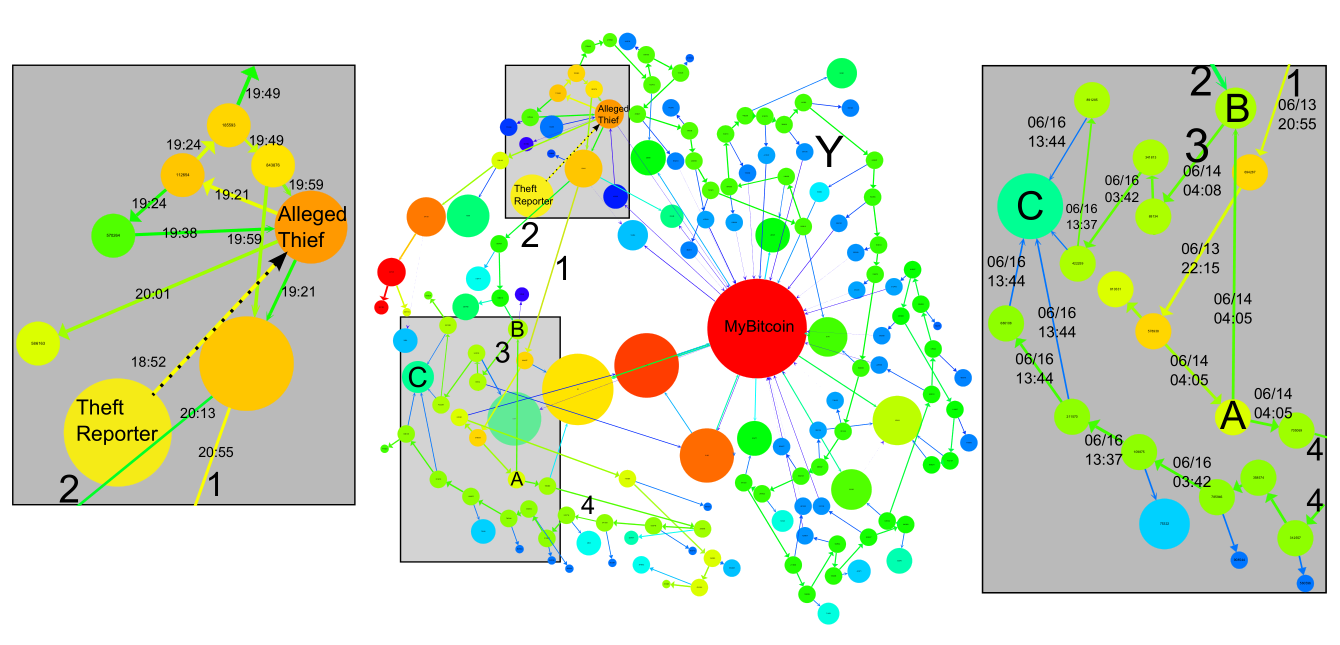
\includegraphics[width=\textwidth]{anonimato_1_13.PNG}
\end{figure}
\end{frame}




%%%%%%%%%%%%%%%%%%%%%%%%%%%%%%%%%%%%%%%%%%%%%%%%%%%%%%%%%%%%%%%%%%%%%%%%%%%%%%%%%%%%
% \item Formula che appare un poco per volta:
% \pause
% \parstepwise{
% $$
%   1\step{{}+2}
%   \step{{}+3} \step{{}+4}\step{{}+\cdots+n}
%   \step{{}={}}
%   \step{\sfondogiallo{$\displaystyle\frac{n(n+1)}{2}$}}
% $$
% }
%
%\pageTransitionGlitter{0}
% il comando \newframe e' come \newpage,
% ma non avanza il numero di pagina.
% Puo' servire per fare cambiamenti incrementali
% a una pagina, quando \pause o \stepwise non
% bastano. In questo esempio \pause non va bene
% perche' qui bisogna aggiungere un paragrafo
% ma allo stesso tempo  cambiare la figura che
% sta in cima alla pagina. Macchinoso da scrivere,
% ma puo' valerne la pena.
%
%\newframe
%
%\sfondogiallo{\rosso{\textit{coincidono:}}}
%
% Le transizioni si attivano al /pause
%\pageTransitionWipe{0}
%\pageTransitionWipe{180}
%\pageTransitionSplitVO
%\item {\setlength{\baselineskip}{2\baselineskip}
%Vedere la documentazione del pacchetto \textcolor{darkorange}{\texttt{texpower}}.
%}
%\pageTransitionReplace
%\pageTransitionBoxI
%%%%%%%%%%%%%%%%%%%%%%%%%%%%%%%%%%%%%%%%%%%%%%%%%%%%%%%%%%%%%%%%%%%%%%%%%%%%%%%%%%%%
\end{document}